\documentclass[11pt]{article}
 
\usepackage[text={6in,8.1in},centering]{geometry}
 
\usepackage{enumerate}
\usepackage{amsmath,amsthm,amssymb}
 
\usepackage{pstricks}
\usepackage{pst-solides3d}
\usepackage{pstricks-add}
\usepackage{graphicx}
\usepackage{pst-tree}
\usepackage{pst-poly}
\usepackage{calc,ifthen}
\usepackage{float}\usepackage{multicol}
\usepackage{multirow}
\usepackage{array}
\usepackage{longtable}
\usepackage{tikz}
\usepackage{tkz-berge}
\usepackage{fancyhdr}
\usepackage{algorithmicx,algpseudocode}
\usepackage{changepage}
\usepackage{color}
\usepackage{listings}
\usepackage{fancyvrb}

\lstset{ %
language=C++,                % choose the language of the code
basicstyle=\footnotesize,       % the size of the fonts that are used for the code
numbers=none,                   % where to put the line-numbers
numberstyle=\footnotesize,      % the size of the fonts that are used for the line-numbers
stepnumber=1,                   % the step between two line-numbers. If it is 1 each line will be numbered
numbersep=5pt,                  % how far the line-numbers are from the code
backgroundcolor=\color{white},  % choose the background color. You must add \usepackage{color}
showspaces=false,               % show spaces adding particular underscores
showstringspaces=false,         % underline spaces within strings
showtabs=false,                 % show tabs within strings adding particular underscores
frame=none,           % adds a frame around the code
tabsize=2,          % sets default tabsize to 2 spaces
captionpos=b,           % sets the caption-position to bottom
breaklines=true,        % sets automatic line breaking
breakatwhitespace=false,    % sets if automatic breaks should only happen at whitespace
escapeinside={\%*}          % if you want to add a comment within your code
}

\newenvironment{block}{\begin{adjustwidth}{1.5cm}{1.5cm}\noindent}{\end{adjustwidth}}

\newtheorem{proposition}{Proposition}[section]
\newtheorem{theorem}{Theorem}[section]
\newtheorem{lemma}{Lemma}[section]
\newtheorem{corollary}{Corollary}[section]
\theoremstyle{definition}
\newtheorem{definition}{Definition}[section]
 
\title{Extremal Functions on Cayley Digraphs of Finite Cyclic Groups \footnote{Supported in part by National Science Foundation (NSF).}}
\author{Jordan Blocher\thanks{Department of Mathematics, University of Nevada-Reno, Reno, NV, USA}\and Samantha Hampton\thanks{Department of Mathematics, University of Arkansas, Fayetteville, AR, USA}\and Christopher Linden\thanks{Department of Mathematics, University of California Los Angeles, Los Angeles, CA,USA } }
\date{\today}
 
 
\def\R{\mbox{$\mathbb R$}}
\def\Q{\mbox{$\mathbb Q$}}
\def\Z{\mbox{$\mathbb Z$}}
\def\N{\mbox{$\mathbb N$}}
\def\C{\mbox{$\mathbb C$}}
\def\Sym{\operatorname{Sym}}
\def\lcm{\operatorname{lcm}}
\def\adj{\operatorname{adj}}
\def\inc{\operatorname{inc}}
\def\Cay{\operatorname{Cay}}
\def\Geom{\operatorname{\cal G}}
\def\ker{\operatorname{ker}}
\def\kernel{\operatorname{ker}}
\def\automorphism{\operatorname{Aut}}
\def\endomorphism{\operatorname{End}}
\def\inner{\operatorname{Inn}}
\def\outer{\operatorname{Out}}
\def\crossing{\operatorname{cr}}
\def\cent{\textcent}
\def\n{\\ \vspace{1.7mm}}
\def\diam{\operatorname{diam}}

\renewcommand{\emptyset}{\O}
 
 
\newcounter{ZZZ}
\newcounter{XXX}
\newcounter{XX}
 
\headsep25pt\headheight20pt
 
 
\pagestyle{fancyplain}
\lhead{\fancyplain{}{\small\bfseries Blocher, Hampton, Linden,\ \ Cayley Digraphs of Finite Cyclic Groups}}
\rhead{\fancyplain{}{\small\bfseries\thepage}}
\cfoot{\ \hfill\tiny\sl Draft printed on \today}
 
 
\setlength{\extrarowheight}{2.5pt} % defines the extra space in tables
 
 
 
\begin{document}
 
\baselineskip6mm\parskip4mm

\maketitle

\begin{abstract}
For positive integers $d$ and $k$ let $m(d,k)$ be defined to be the maximum modulus m such that the \emph{Cayley digraph} Cay($\Z_{m}, \mathcal{A}$) generated by the set of positive integers $\mathcal{A}$ of cardinality $k$ is such that the diameter of Cay($\Z_{m}, \mathcal{A}$) is less than or equal to $d$. 
In this paper we give a construction which establishes a new lower bound for $m(2, k)$, and then use this to obtain an asymptotic lower bound for the general case $m(d,k)$.
\end{abstract}
 
\pagebreak

\section{Introduction}
\subsection{Cayley Digraphs and Extremal Bases} 
Let $\Gamma$ be a finite group with a subset $\mathcal{A}$. The \emph{Cayley digraph}, denoted Cay($\Gamma, \mathcal{A}$), is a digraph with vertex set $\Gamma$, such that ($x, y$) is a directed edge if and only if $yx^{-1}$ $\in$ $\mathcal{A}$.
The focus of this paper is the finite group $\Z_m$; we will denote the Cayley digraph Cay($\Z_m, \mathcal{A}$) as Cay($m, \mathcal{A}$).

 \begin{figure}[h]
\begin{center}

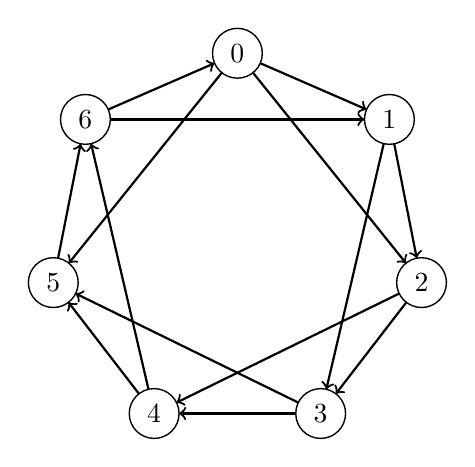
\begin{tikzpicture}

\Vertex[x=187.5pt,y=255.44534805153816pt]{0};
\Vertex[x=242.42118923300023pt,y=231.541497539934pt]{1};
\Vertex[x=254.03680848710601pt,y=172.5735690432419pt]{2};
\Vertex[x=217.58400229878092pt,y=125.26840951092518pt]{3};
\Vertex[x=157.4159977012192pt,y=125.26840951092518pt]{4};
\Vertex[x=120.96319151289404pt,y=172.57356904324183pt]{5};
\Vertex[x=132.57881076699977pt,y=231.541497539934pt]{6};
\tikzset{EdgeStyle/.style={->}}
\Edge(1)(2)
\Edge(0)(1)
\Edge(6)(0)
\Edge(5)(6)
\Edge(4)(5)
\Edge(3)(4)
\Edge(2)(3)
\Edge(0)(2)
\Edge(2)(4)
\Edge(4)(6)
\Edge(6)(1)
\Edge(1)(3)
\Edge(3)(5)
\Edge(0)(5)
\end{tikzpicture}
\end{center}
\caption{ Cay($\Z_7$, \{1,2\}).}
\end{figure}
The Cayley digraph of a finite cylic group is called a circulant graph. Cayley digraphs, and circulant graphs in particular are often used as models for interconnection networks. As such, it is natural to want to maximize the number of vertices which can be connected with constraints on diamter and degree.
For any positive integer $d$ we define
\[
m(d,\mathcal{A}) =\ \max\{m \  \vert \  \diam(Cay(m,\mathcal{A})) \leq d\},
\]
the largest positive integer $m$ such that the diameter, $d(m,\mathcal{A})$, of the Cayley digraph $Cay(m,\mathcal{A})$ is less than or equal to $d$. For positive integers $d$ and $k$,
\[
m(d, k) = \max_{\scriptstyle \mathcal{A}\subseteq\mathbb Z^{+}\atop\scriptstyle |\mathcal{A}|=k}\{m\  |\  \diam(Cay(m,\mathcal{A})) \leq d\}
\]
the maximum modulus $m$ such that there exists a generating set with cardinality equal to $k$ and the diameter of the Cayley digraph is less than or equal to $d$. 
$\\$

Current known values include
\begin{align*}
m(1,k)& = k+1,\\
m(d,1) &= d+1\text{, and}\\
m(d,2) &=\left \lfloor \frac{d(d+4)}{3}\right \rfloor+1 \text{ for all } d\geq2. \cite{JiaHsu}
\end{align*}

\subsection{The Postage Stamp Problem}
 Let $d$ be a positive integer. We define $n(d, k)$ to be the largest positive integer $n$ such that there exists a subset $\mathcal{A}$ of positive integers with the property that every integer in the interval $[1, n]$ is the sum of at most $d$ not necessarily distinct elements of $\mathcal{A}$. In other words, 
\[
n(d, k) = \max_{\scriptstyle \mathcal{A}\subseteq\mathbb Z^{+}\atop\scriptstyle |\mathcal{A}|=k}\{n\  |\ d\cdot \mathcal{A}\supseteq[1, n]\}.
\]
The computation of  $n(d, k)$ is often referred as the \emph{postage stamp problem}. The postage stamp problem is an old problem in number theory that has been studied extensively. See  for more information. Any basis $\mathcal{A}$ for $[1, n]$ is also a basis for $\Z_n$, so for all positive $d$ and $k$ we have $m(d, k) \geq n(d, k)$.

The  best known lower bound for $n(2,k)$ was proved by Mrose \cite{Mrose1979}
\[
n(2, k) \geq \frac{2}{7}k^2 + \frac{12}{7}k + O(1)\qquad  \text{as}\quad  k \to \infty.
\]
Together with the inequality $m(d, k) \geq n(d, k)$, this lower bound gives a trivial lower bound on $m(2, k)$ which was the best known. We prove a non-trivial lower bound for $m(2,k)$ in the following theorem.

 
\section{New Lower Bound of $m(2, k)$.}
\subsection{Main Result}

 
\begin{theorem}
$\displaystyle m(2,k) \geq \frac{37}{121}k^2 + O(k)$  as $ k \to \infty$.
\end{theorem}

\begin{proof}
Let $k \geq$ 14 be an integer. Let $\displaystyle k_1 = \left \lfloor \frac{k - 3}{11} \right \rfloor$. Let $m = 37k_1^2$.  Define 
\begin{align*}
I_\mu &= [\mu k_1^2, \mu k_1^2 + k_1],
&&\mu = 0, 4, 15, 26; \\
S_\nu &= \{\nu k_1^2 + ik_1 \ |\  i = 0 , 1, ... , k_1 - 1\},
&&\nu = 0, 1, 2, 3;\\
T_{\eta} &= \{\eta k_1^2+ i(k_1 + 1) \ |\   i = 0 , 1, ... , k_1 -1\},
&&\eta = 10, 20, 30.
\end{align*}
 Let $S= S_{0} \cup S_{1} \cup S_{2} \cup S_{3}$, and
define
\[
\mathcal{A}=I_0\cup I_4\cup I_{15}\cup I_{26}\cup S\cup T_{10}\cup T_{20}\cup T_{30}.
\]
Noting  that $I_0\cap S_0=\{0\}$, and 
\[
|I_\mu| = k_1 + 1,\quad 
|S_\nu| = k_1,\quad\text{and}\quad
|T_\eta| = k_1,
\]
we see that 
\[
|\mathcal{A|} \leq 11k_1 + 3 \leq k.
\]  
We now prove that $\mathcal{A}+\mathcal{A}=\Z_m$.
We begin by claiming $I_{\mu}+T_{\eta}\supseteq[(\mu + \eta )k_1^2 ,  (\mu + \eta  + 1)k_1^2)$. Let $n \in[(\mu + \eta )k_1^2 ,  (\mu + \eta  + 1)k_1^2)$.
Then we can write $n$ as 
\[
n = (\mu + \eta ) k_1^2 + qk_1 + r,
\]
where $0 \leq q < k_1$ and $0 \leq r < k_1$.

If $r \geq q$, then $0\le r-q<k_{1}$ and
\[
n = \mu k_1^2 +  (r - q)+ \eta k_1^2 + q(k_1+1).
\]
 Since 
 \[
 \mu k_1^2 + (r - q) \in I_\mu\qquad\text{and}\qquad \eta k_1^2 +q(k_1+1) \in T_\eta,
 \]
we see that $n \in I_{\mu}+T_{\eta}$. 

If $r < q$, then we must have $q \geq 1$ and $0\le k_{1}+r-q+1\le k_{1}$. Then
\[
\mu k_1^2 + (k_1 + r - q + 1) \in I_\mu \qquad \text{and}\qquad
\eta k_1^2 + (q - 1)(k_1 + 1) \in T_\eta.
\]
 Hence
\[
n = \mu k_1^2 + (k_1 + r - q + 1)+\eta k_1^2 + (q - 1)(k_1 + 1) \in I_{\mu}+T_{\eta}.
\]
 

Next we claim that  $I_{\mu}+S_{\nu}\supseteq[(\mu + \nu )k_1^2 ,  (\mu + \nu  + 1)k_1^2)$. Let $n \in[(\mu + \nu )k_1^2 ,  (\mu + \nu  + 1)k_1^2)$.
Then we can write $n$ as 
\[
n = (\mu + \nu ) k_1^2 + qk_1 + r = \mu k_1^2 + r+\nu k_1^2 + qk_1,
\]
where  $0 \leq q < k_1$ and $0 \leq r < k_1$, such that 
\[
\mu k_1^2 + r \in I_\mu \qquad\text{and}\qquad\nu k_1^2 + qk_1 \in S_\nu,
\]
 so $n \in I_{\mu}+S_{\nu}$. 

Our final claim is $S+T_\eta \supseteq[(\eta  +1)k_1^2 ,  (\eta  + 4)k_1^2)$.  Let $n \in[(\eta  +1)k_1^2 ,  (\eta  + 4)k_1^2)$.
Then we can write $n$ as 
\[
n = (\eta  + \nu ) k_1^2 + qk_1 + r, 
\]
where $1 \leq \nu  \leq 3$, $0 \leq q < k_1$, and $0 \leq r < k_1$. 

If $q \geq r$, then
\[
n = \nu k_1^2 + (q - r) k_1+\eta k_1^2 + r(k_1 + 1), 
\]
where $\nu k_1^2 + (q - r)k_1 \in S_\nu$ and $\eta k_1^2 + d(k_1 + 1) \in T_\eta$, so $n \in S_\nu +T_\eta$. 

If $q <r$, then
\[
n = (\nu  - 1)k_1^2 + (k_1 + q - r) k_1+\eta k_1^2 + r(k_1 + 1), 
\]
where 
\[
(\nu  - 1)k_1^2 + (k_1 + q - r)k_1 \in S_{\nu  - 1}\qquad\text{and}\qquad
\eta k_1^2 + r(k_1 + 1) \in T_\eta.
\]
Hence $n \in S_{\nu-1}+T_\eta\subseteq S+T_{\eta}$. 
It is clear that, in $\Z_{37k_{1}^{2}}$,
\begin{align*}
[45k_{1}^{2},46k_{1}^{2})&=[8k_1^2, 9k_1^2),\\
[46k_{1}^{2},47k_{1}^{2})&=[9k_1^2, 10k_1^2),\\
[56k_{1}^{2},57k_{1}^{2})&=[19k_1^2, 20k_1^2).
\end{align*}
Therefore, we have proved that the entire interval $[0, m)=\Z_{m}$ can be  {\em covered\/} as follows: 
\begin{align*}
I_0 + S  &\supseteq [0, 4k_1^2),\\
I_4 + S  &\supseteq [4k_1^2, 8k_1^2),\\
I_{15} + T_{30}  &\supseteq[45k_{1}^{2},46k_{1}^{2})= [8k_1^2, 9k_1^2),\\
I_{26} + T_{20}  &\supseteq[46k_{1}^{2},47k_{1}^{2})= [9k_1^2, 10k_1^2),\\
I_{0}+T_{10}  &\supseteq [10k_1^2, 11k_1^2),\\
S+T_{10}  &\supseteq [11k_1^2, 14k_1^2),\\
I_{4} + T_{10}  &\supseteq [14k_1^2, 15k_1^2),\\
I_{15} + S  &\supseteq [15k_1^2, 19k_1^2),\\
I_{26} + T_{30}  &\supseteq[56k_{1}^{2},57k_{1}^{2})= [19k_1^2, 20k_1^2),\\
I_{0} + T_{20}  &\supseteq [20k_1^2, 21k_1^2),\\
S + T_{20}  &\supseteq [21k_1^2, 24k_1^2),\\
I_{4} + T_{20}  &\supseteq [24k_1^2, 25k_1^2),\\
I_{15} + T_{10}  &\supseteq [25k_1^2, 26k_1^2),\\
I_{26} + S  &\supseteq [26k_1^2, 30k_1^2),\\
I_{0} + T_{30}  &\supseteq [30k_1^2, 31k_1^2),\\
S + T_{30}  &\supseteq [31k_1^2, 34k_1^2),\\
I_{4} + T_{30}  &\supseteq [34k_1^2, 35k_1^2),\\
I_{15} + T_{20}  &\supseteq [35k_1^2, 36k_1^2),\\
I_{26} + T_{10}  &\supseteq [36k_1^2, 37k_1^2).
\end{align*}
It now follows that 
\[
\mathcal{A} + \mathcal{A} \supseteq [0, 37k_1^2).
\]
Hence
\begin{align*}
m(2,k) &\geq 37k_1^2\\
&= 37 \cdot \left \lfloor \frac{k - 2}{11}\right \rfloor^2\\
&> 37 \left(\frac{k - 2}{11} -1\right) ^2\\
&= \frac{37}{121}k^2-\frac{962}{121}k+\frac{6253}{121}\\
&= \frac{37}{121}k^2 + O(k)\qquad \text{ as }\quad k \to \infty. \qedhere
\end{align*}
\end{proof}
\subsection{General Case}
As a corollary, we use the inequality 
\[
m(d_1+d_2,k_1+k_2) \geq m(d_1,k_1)m(d_2,k_2)
\]
for $d_1, d_2 \geq 1$ and $k_1, k_2 \geq 2$ to establish a lower bound for $m(d,k)$ for fixed $d$ as $k \to \infty$.
\begin{theorem}
For $d \geq 2$, as $k \to \infty$ 
\[
m(d,k) \geq \left(\frac{148}{121}\right)^{\lfloor \frac{d}{2}\rfloor}\left(\frac{k}{d}\right)^d + O(k^{d-1}).
\]
\end{theorem}
\begin{proof}
Let $d = 2q +r$ where $q = \lfloor \frac{d}{2}\rfloor$ and $k = du +v$ where $u = \lfloor \frac{k}{d}\rfloor$.

Then 
\begin{align*}
m(d,k) &= m(2q+r, du +v)\\
&= m(2q+r, (2q+r)u +v)\\
&\geq m(2q, 2qu) \geq m(2, 2u)^q\\
&\geq \left(\frac{37}{121}(2u)^2+ O(2u)\right)^q \\
&= \left(\frac{148}{121} \left(\frac{k-v}{d}\right) ^2+ O(2u)\right)^{\lfloor \frac{d}{2}\rfloor}\\
&= \left(\frac{148}{121}\right)^{\lfloor \frac{d}{2}\rfloor}\left(\frac{k}{d}\right)^d + O(k^{d-1})
\end{align*}
\end{proof}
\section{Remarks and Open Problems}

We used a computer program to test candidates for the values that appeared in the proof as the subscripts $\mu,\ \nu$ and $\eta$.  It is likely that our result could be improved upon by a more complicated construction using a larger number of the same types of subsets.  However, testing larger constructions becomes computationally difficult, and there is a theoretical limit of $1/3$ on the leading coefficient of such a construction.

There are many results for $n(d,k)$ for which analogous results about $m(d,k)$ have not been proved.
For $n(d,k)$ it is known that for every positive integer $k$ the limit 
\[
\lim_{d \to \infty}{\frac{n(d,k)}{d^k}}
\]
exists, and the value is known for $k = 1,$ $2$ and $3$.  It is not known whether or not 
\[
\lim_{d \to \infty}{\frac{m(d,k)}{d^k}}
\]
exists for every k, and the value is only known for $k = 1$ and $2$. The case where $k$ is variable and $d$ is fixed is relatively unstudied.

\newpage
\bibliographystyle{plain}	
\bibliography{myrefs}		

\end {document}

